\documentclass{article}
\usepackage[portuguese]{babel}
\usepackage[utf8]{inputenc}
\usepackage{amsmath}
\usepackage{amssymb}
\usepackage{graphicx}
\usepackage{caption}
\usepackage{float}
\usepackage{subcaption}
\usepackage{pdflscape}
\usepackage{multirow}
\usepackage[table,xcdraw]{xcolor}

\author{Cláudio Ferreira Carneiro - RA 263796}
\title{EFC 2}
\begin{document}
    \maketitle
    \pagenumbering{gobble}
    \newpage
    \pagenumbering{arabic}
    \section[]{Parte II – Classificação binária com redes MLP e SVMs}
    O código referente às atividades se encontra no repositório:
    
    https://github.com/carneirofc/IA006.git\linebreak
    \subsection*{a)} Antes da inicialização do treinamento,
    os dados de entrada foram redimensionados utilizando o \textit{standard scaler},
    tendo a média removida e escalado à variância unitária, equação \ref{eq:std_scaler}.
    A classe representada por $-1$ passará a ser representada por $0$ a fim de utilizar a
    função de custo \textit{Binary Cross-Entropy} no trinamento do modelo. A figura \ref{fig:out_data_scaled}
    apresenta o histograma das saídas (classes) do \textit{dataset} de treinamento.
    \begin{align}
        z &= (x - \mu) / \sigma
        \label{eq:std_scaler}
    \end{align}
    A figura \ref{fig:inp_data_scaled} apresenta os dados de treinamento de entrada originais e 
    escalados pelo \textit{standard scaler}. Nota-se que não ocorreram mudanças significativas
    no \textit{dataset}.
    \begin{figure}[H]
        \centering
        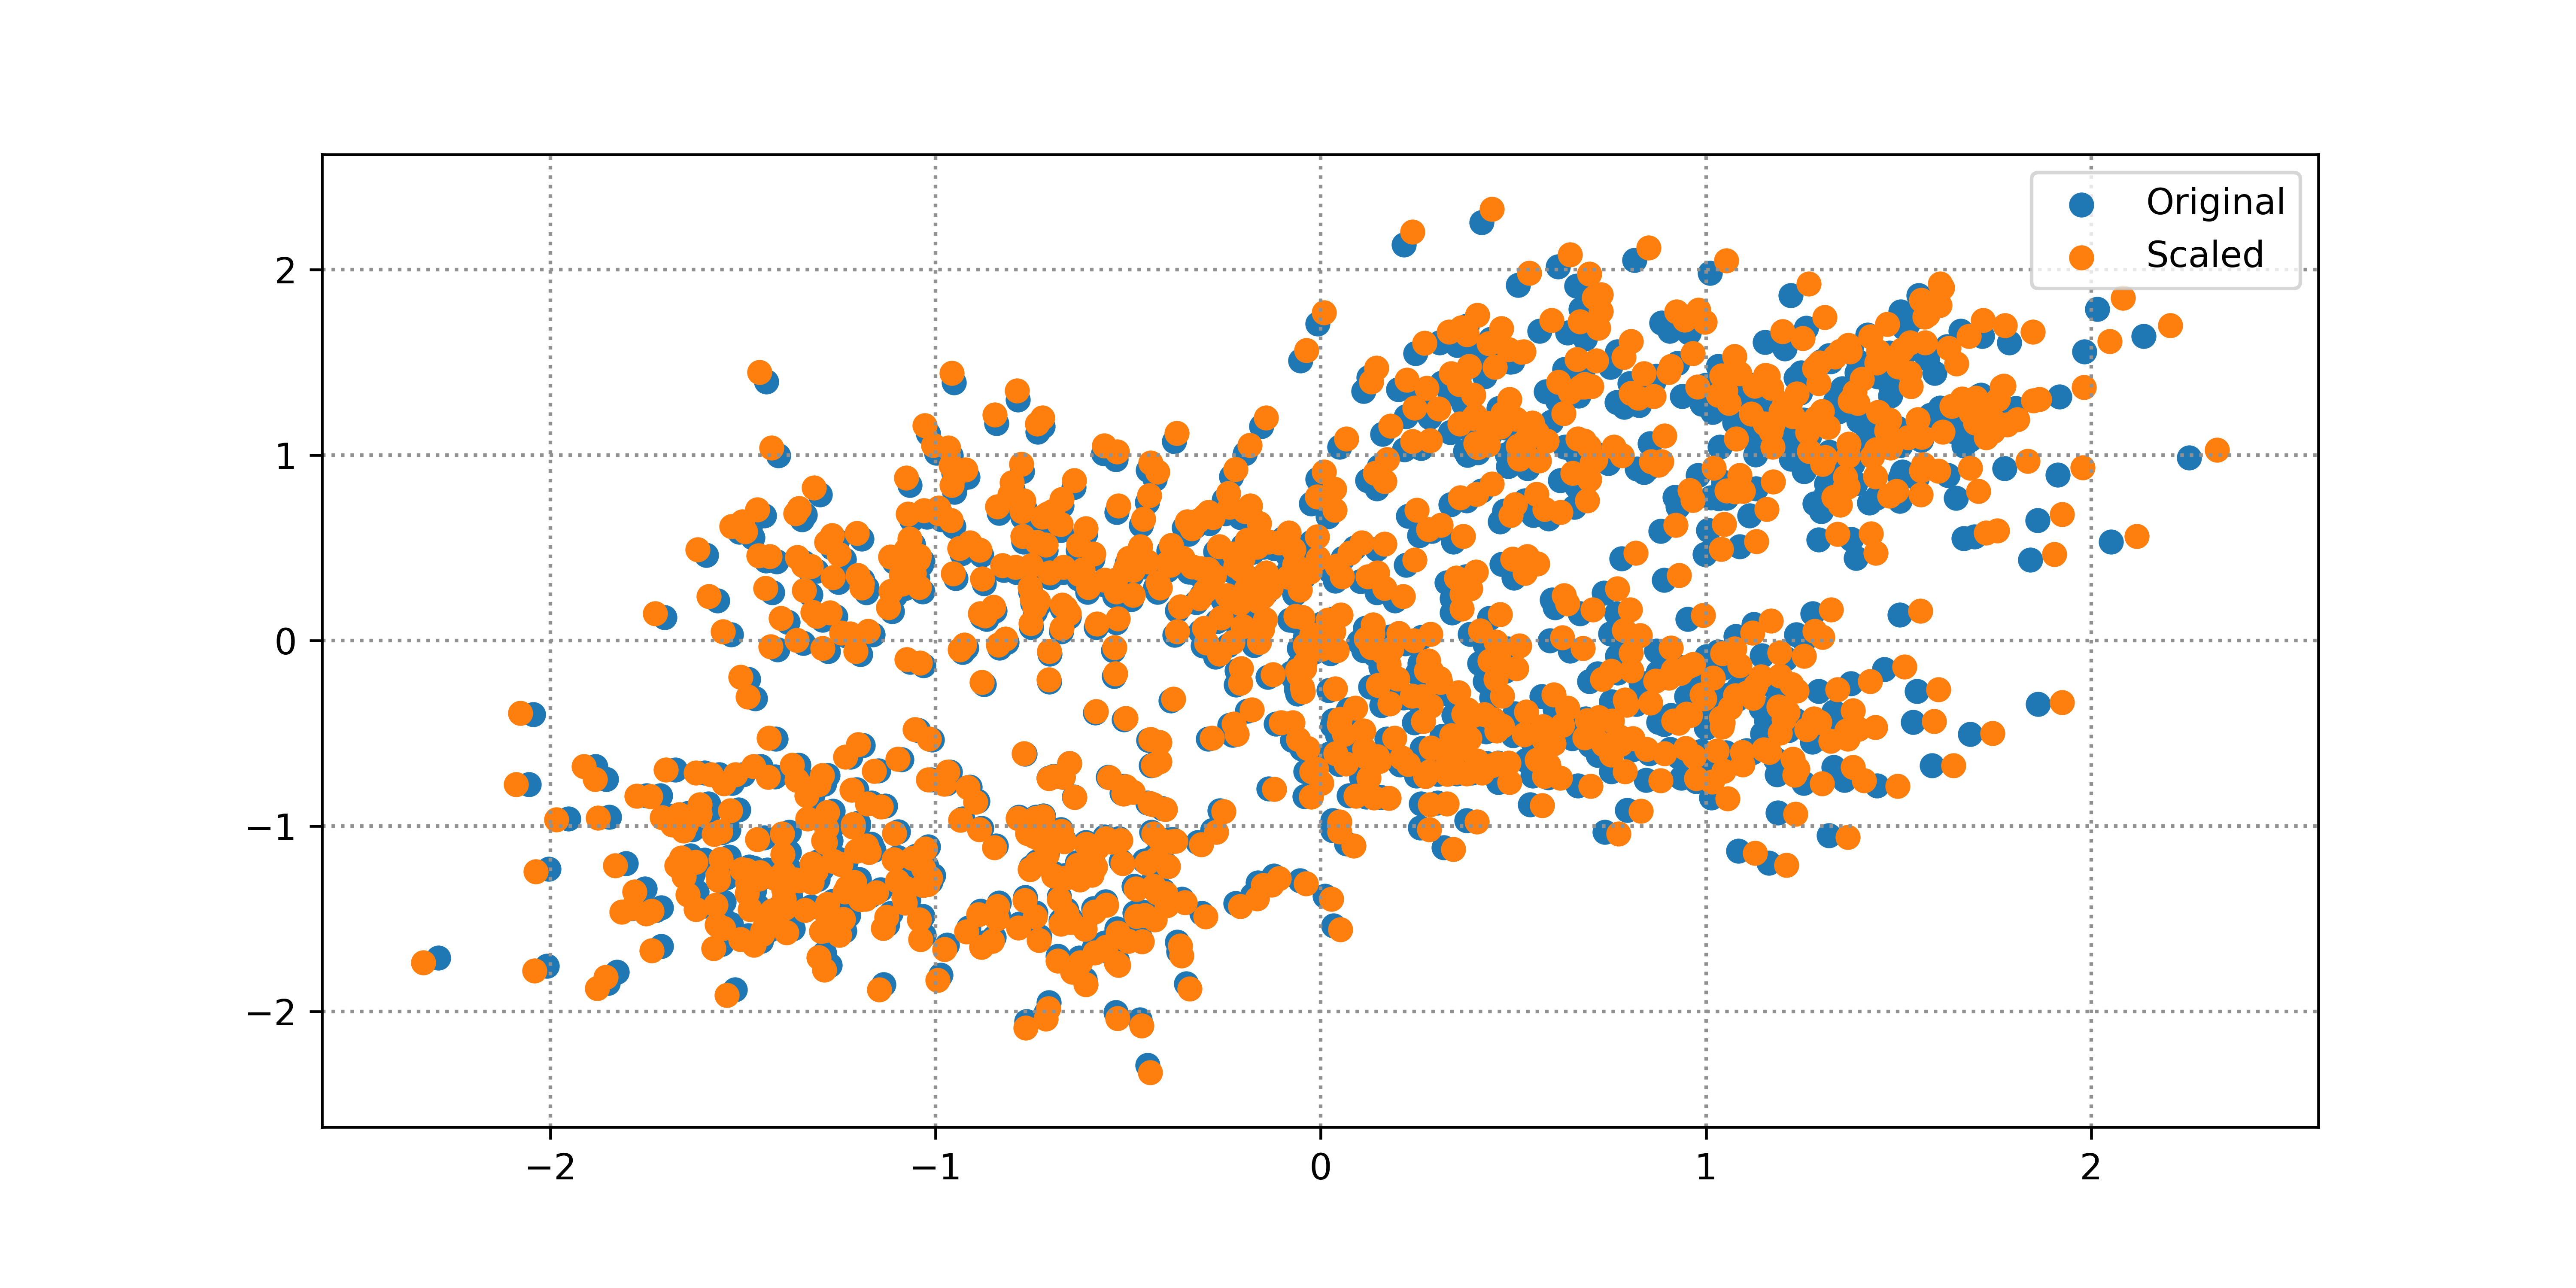
\includegraphics[width=\linewidth]{mlp_inp_scaled.png}   
        \caption{\textit{Dataset} de treinamento, atributos de entrada
            originais e escalados.}
        \label{fig:inp_data_scaled}
    \end{figure}
    
    \begin{figure}[H]
        \centering
        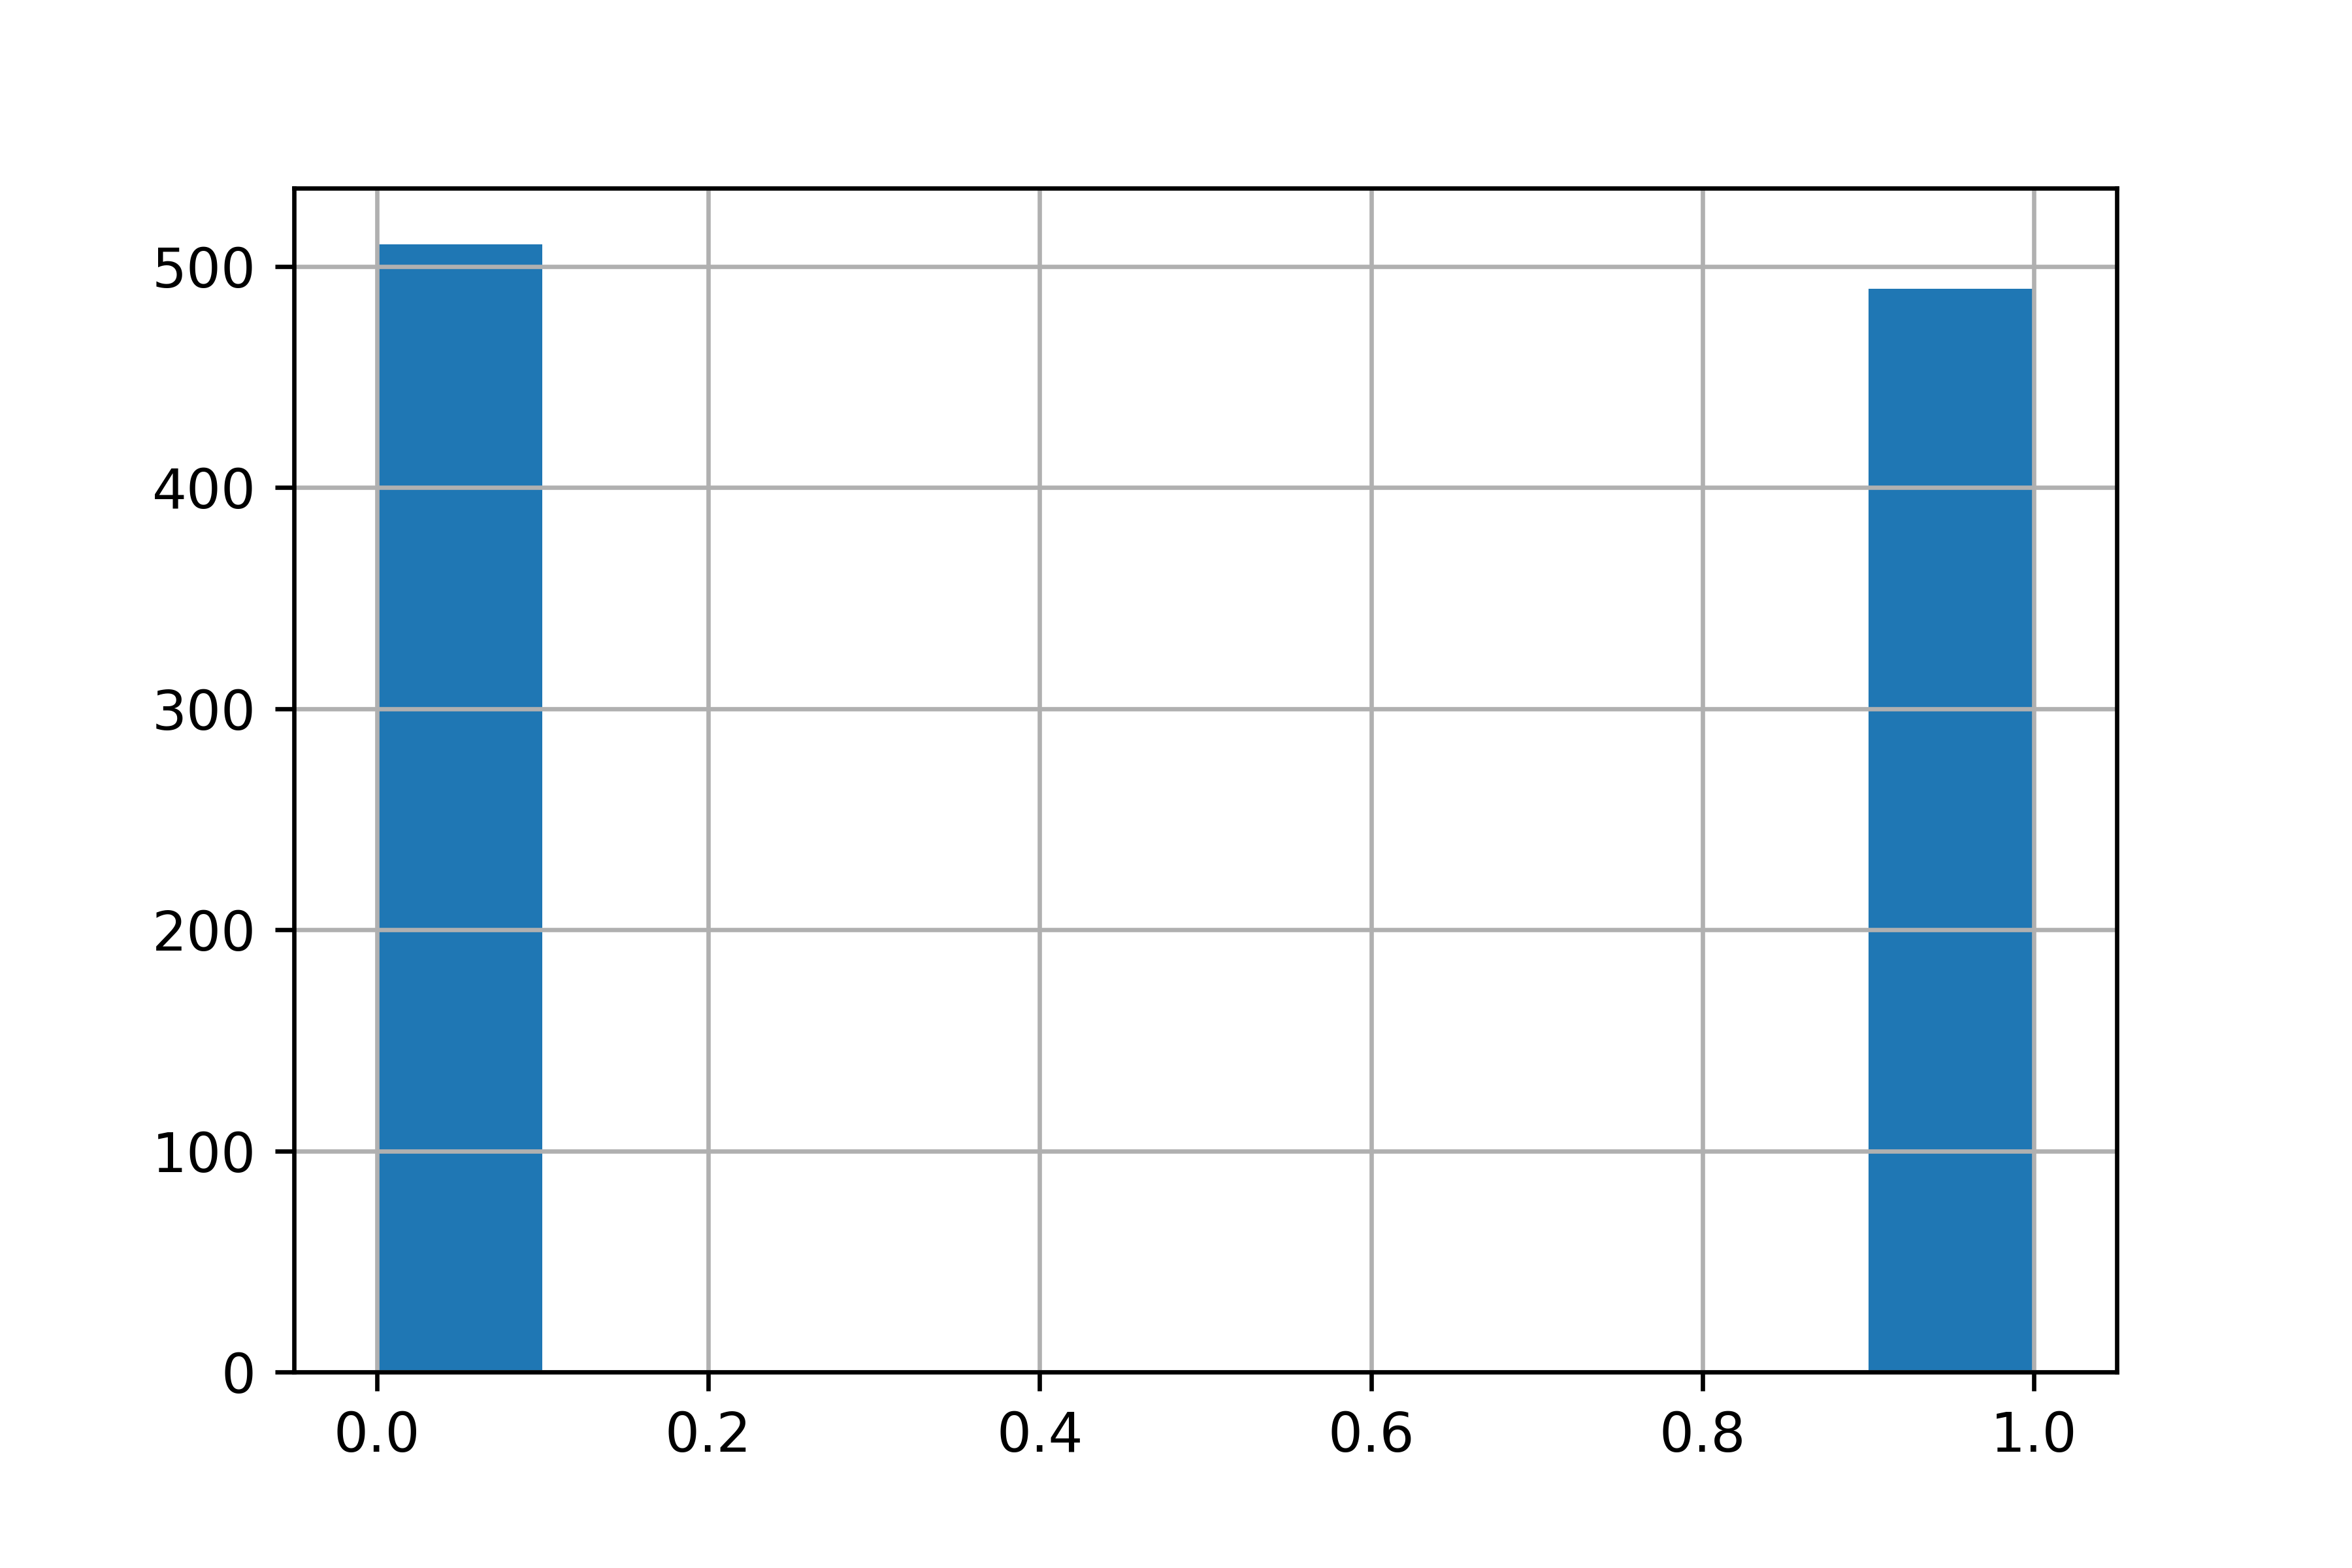
\includegraphics[width=\linewidth]{mlp_out_scaled.png}   
        \caption{\textit{Dataset} de treinamento, classes $0$ e $1$.}
        \label{fig:out_data_scaled}
    \end{figure}
    A MPL foi definida como uma rede de $35$ neurônios na camada intermediária, utilizando
    como função de ativação a \textit{ReLU}. Na camada de saída apenas um neurônio é utilizado,
    cuja função de ativação é a \textit{sigmoid}, equação \ref{eq:sigmoid}.
    O processo de treinamento da MPL utilizou o \textit{RMSprop} como algoritmo de treinamento.
    \begin{align}
        y(x) &= \frac{1}{1 + \exp^{-x}}
        \label{eq:sigmoid}
    \end{align}
    O processo de treinamento foi definido com duração de $1000$ épocas com critérios de 
    parada prematura. Os dados de entrada foram embaralhados e apresentados
    em \textit{batch} com $10$ amostras.
    Como critérios de parada prematura, foram utilizados \textit{snapshots} da configuração de pesos
    de menor custo nos dados de validação e a variação do erro de validação.
    Quando o erro de validação não superar o limiar especificado ($0.001$) por $patience=200$ épocas,
    o treinamento é finalizado.
    
    A MLP foi treinada por $200$ épocas, quando o processo foi interrompido pela
    parada prematura, com custo de treinamento $loss: 0.3236$ e custo de validação
    $val_loss: 0.3471$, figura \ref{fig:mlp_training}. Os pesos utilizados são da época $134$, onde o custo de validação
    é $val_loss: 0.34124$.

    \begin{figure}[H]
        \centering
        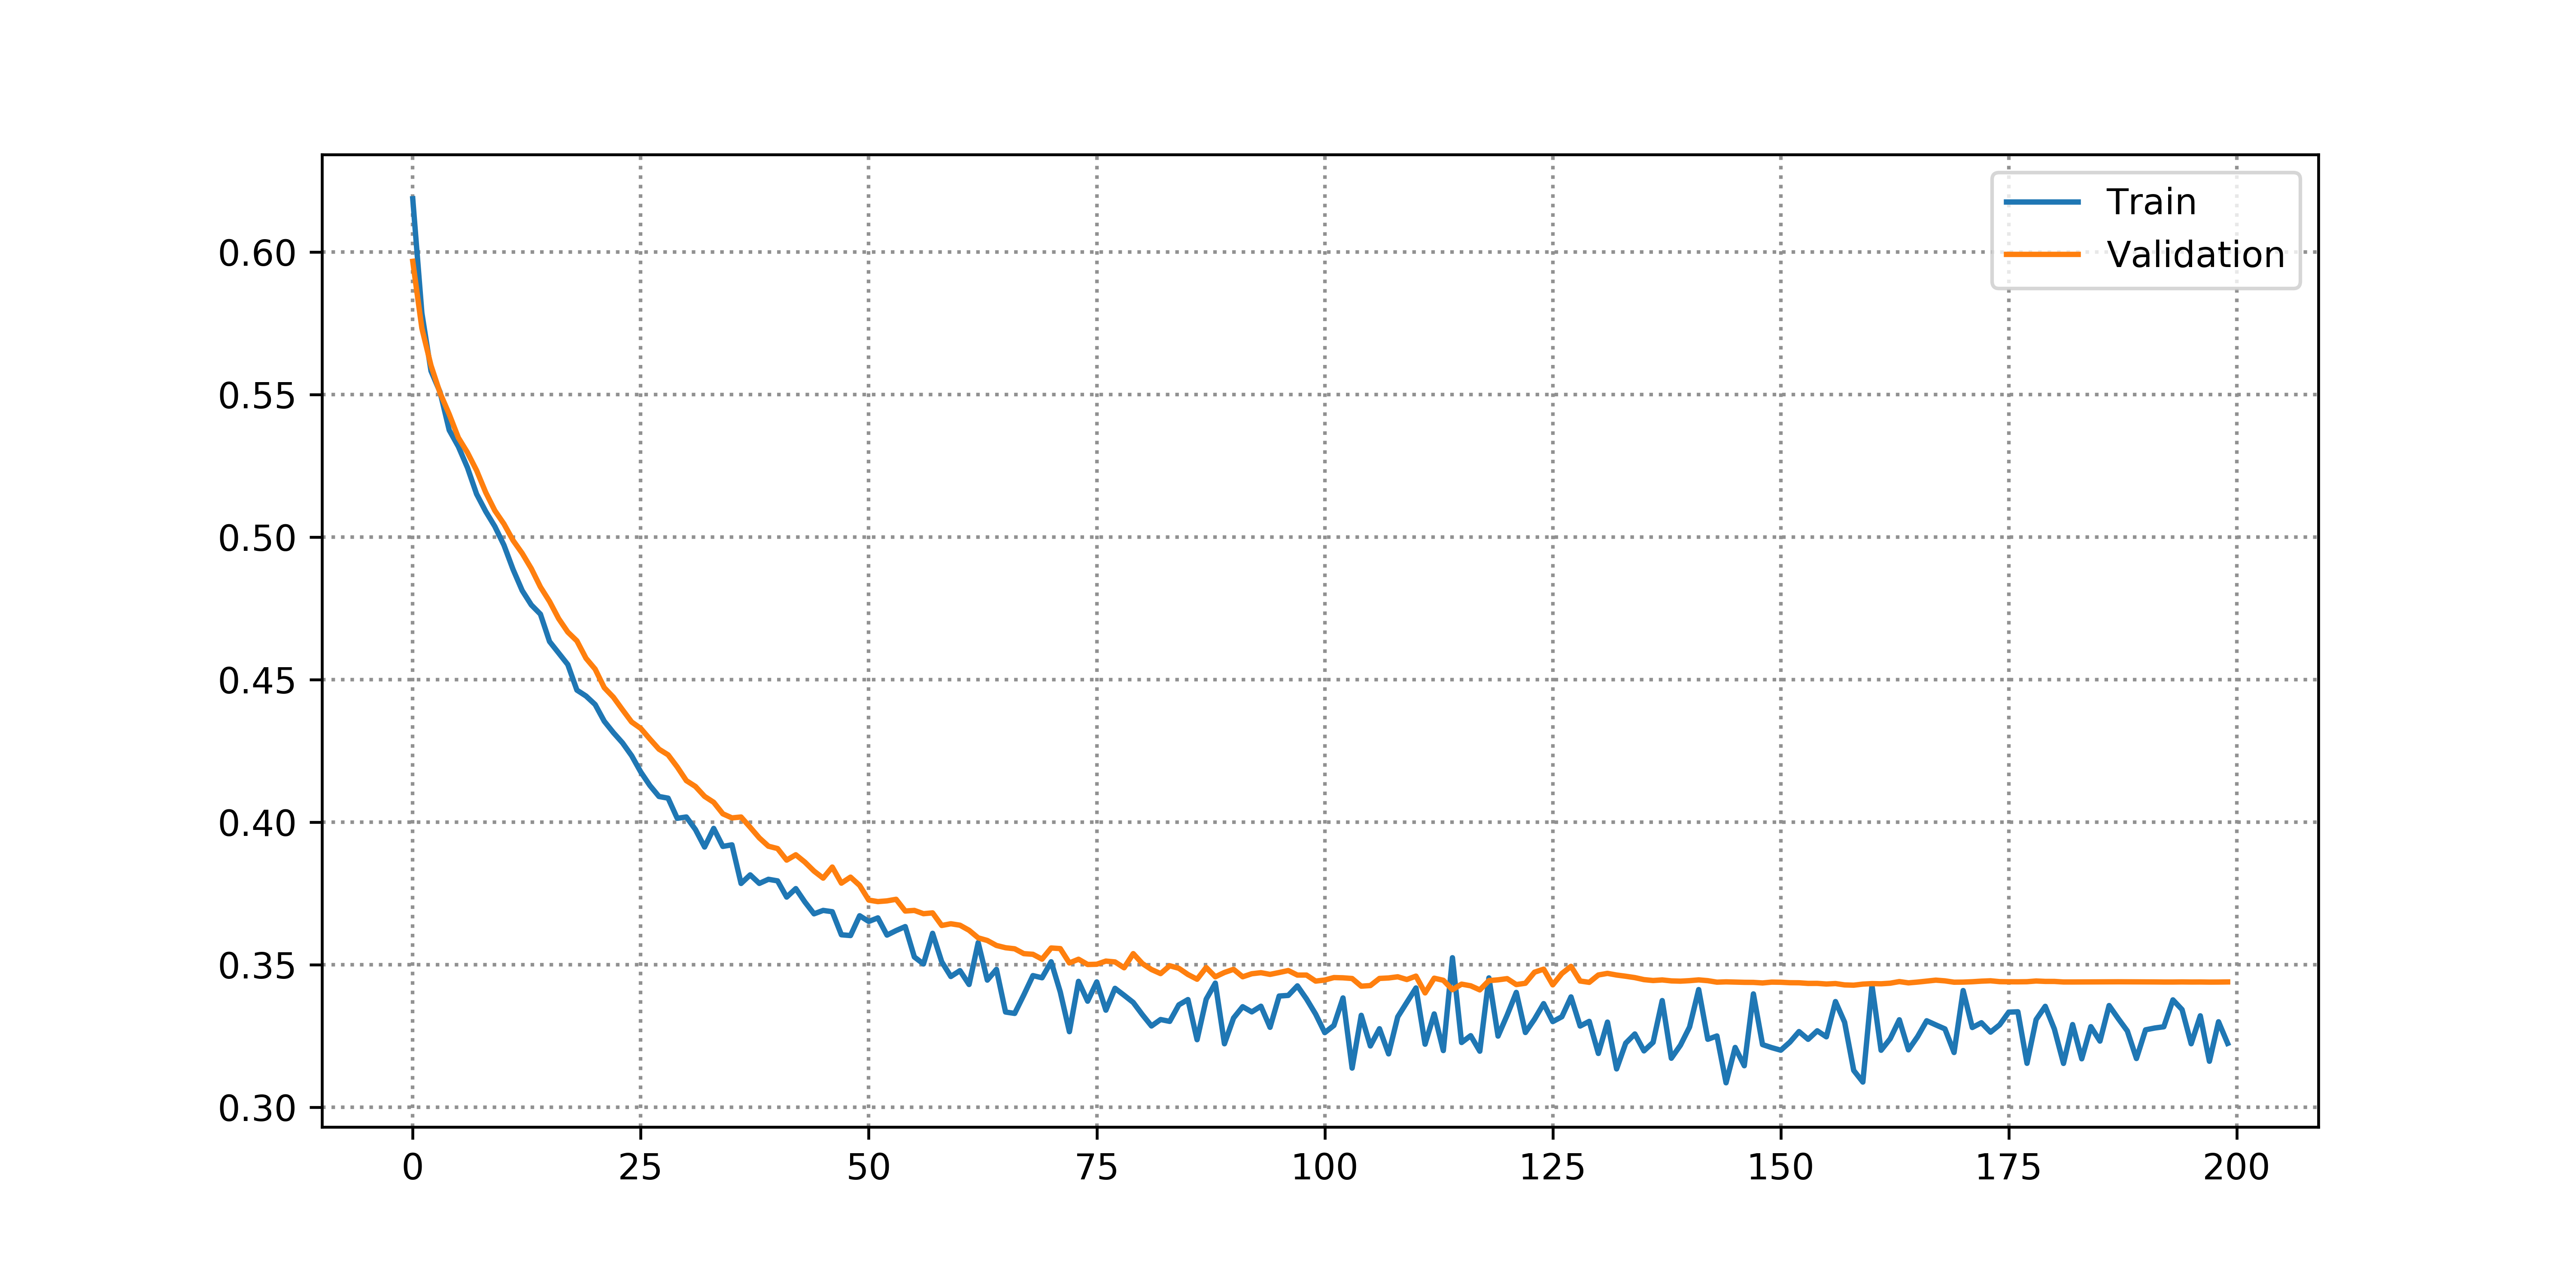
\includegraphics[width=\linewidth]{mlp_training.png}   
        \caption{Histórico de erro no processo de treinamento.}
        \label{fig:mlp_training}
    \end{figure}
   
    A curva ROC da MLP é vista na figura \ref{fig:mlp_roc}, com pontuação de $\approx0.9261$ para os dados de validação.
    \begin{figure}[H]
        \centering
        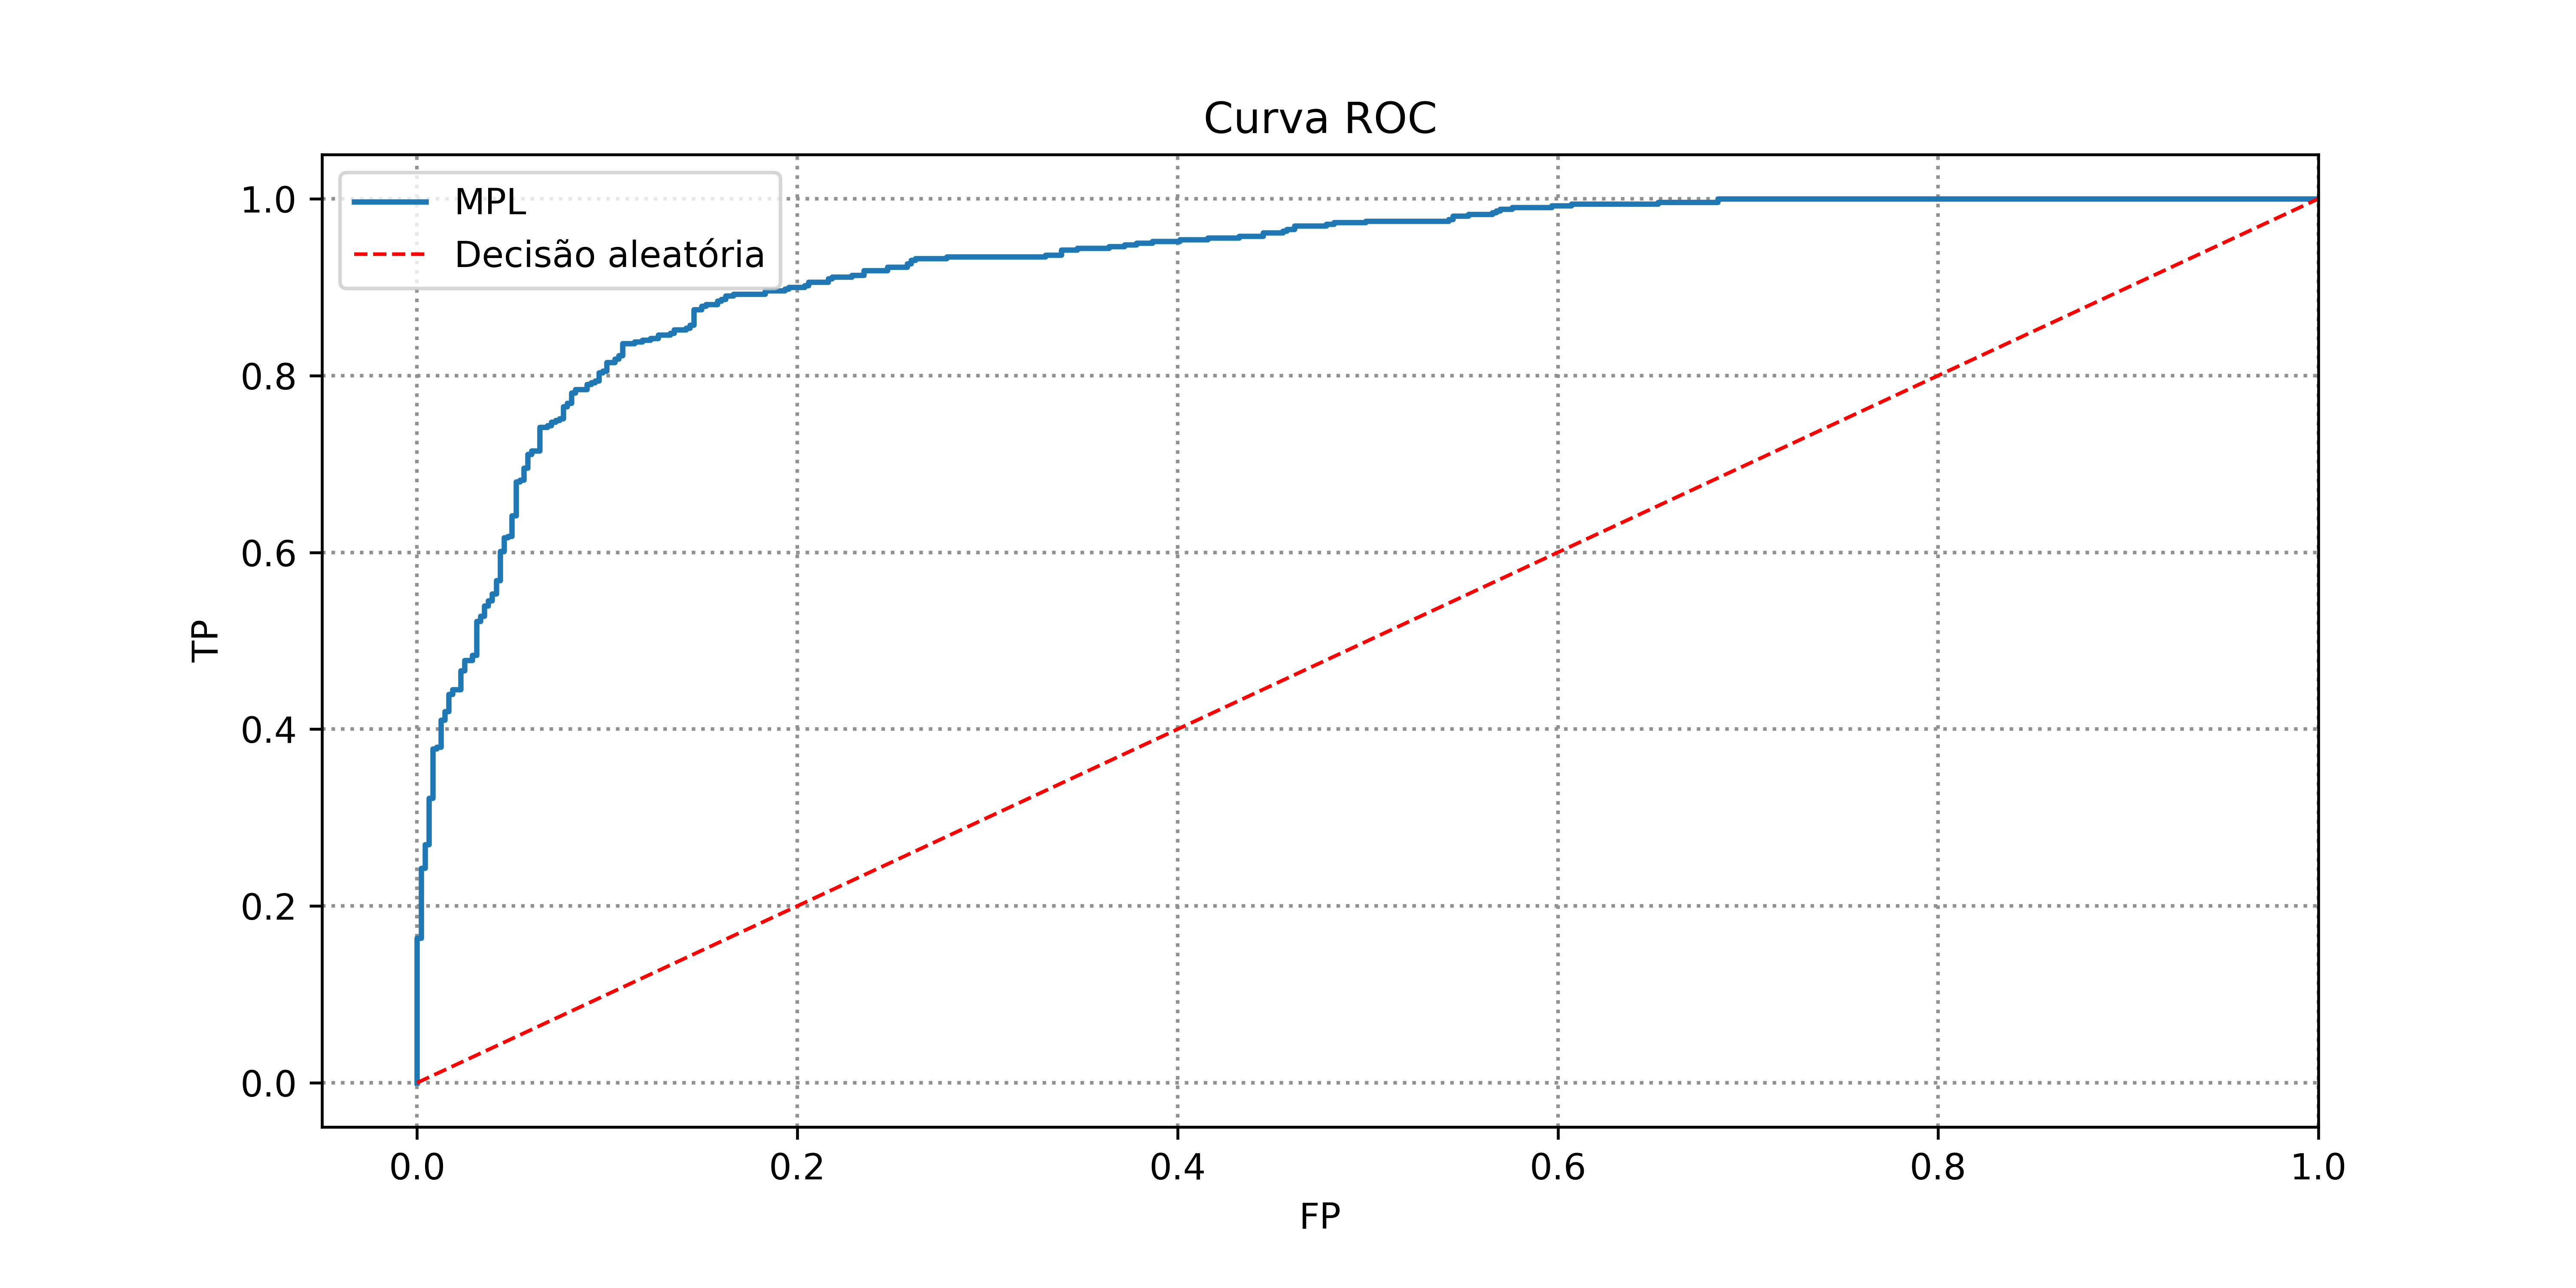
\includegraphics[width=\linewidth]{mlp_roc.png}   
        \caption{Curva ROC da MLP para os dados de validação.}
        \label{fig:mlp_roc}
    \end{figure}

    \subsection*{b)}
    A região de decisão se assemelha à região ótima porém é visível ainda existem padrões
    a serem capturados pela MPL.
    \begin{figure}[H]
        \centering
        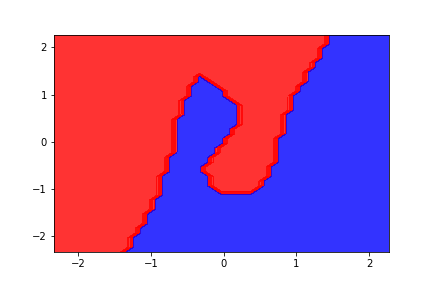
\includegraphics[width=\linewidth]{mpl_decision.png}   
        \caption{Regiões de decisão.}
        \label{fig:mpl_decision}
    \end{figure}

    \subsection*{c)}
    A MPL obteve uma acurácia de $87\%$ como é visto na tabela \ref{tbl:mpl_test}.
    \begin{table}[H]
        \begin{tabular}{c|c|c|c|c|}
        \cline{2-5}
                                        & \textbf{Precision} & \textbf{Recall} & \textbf{f1-score} & \textbf{support} \\ \hline
        \multicolumn{1}{|c|}{Classe -1}    & 0.86               & 0.88            & 0.87              & 499              \\ \hline
        \multicolumn{1}{|c|}{Classe 1}     & 0.88               & 0.86            & 0.87              & 501              \\ \hline
        \multicolumn{1}{|c|}{}             &                    &                 &                   &                  \\ \hline
        \multicolumn{1}{|c|}{accuracy}     &                    &                 & 0.87              & 1000             \\ \hline
        \multicolumn{1}{|c|}{macro avg}    & 0.87               & 0.87            & 0.87              & 1000             \\ \hline
        \multicolumn{1}{|c|}{weighted avg} & 0.87               & 0.87            & 0.87              & 1000             \\ \hline
        \end{tabular}
        \caption{Classificação do \textit{dataset} de teste.}
        \label{tbl:mpl_test}
    \end{table}

    \subsection*{d)}

    \subsection*{e)}

    \subsection*{f)}
    
    \subsection*{g)}

\end{document}